\subsection{Verso la Requirements and Technology Baseline}
\subsubsection{Primo periodo  06/11/2023 - 24/11/2023}
\paragraph{Considerazioni}
    Nel corso del primo periodo, il nostro team ha dedicato risorse significative all'elaborazione e alla standardizzazione dei \textit{processi}\textsubscript{\textit{G}}, formalizzando tali linee guida nel documento \textit{Norme di Progetto}. In quest'ultimo, sono state dettagliatamente redatte le sezioni specificate nella tabella sottostante.

    \vspace{0.2cm}

    Durante il primo incontro con l'azienda, abbiamo definito obiettivi chiave da conseguire entro il prossimo \textit{SAL}\textsubscript{\textit{G}} fissato per il 24 novembre 2023, coincidente con l'avvio del prossimo periodo. Questo approccio ricalca la struttura dello sprint backlog del \textit{framework}\textsubscript{\textit{G}} Scrum. \\
    Tra i molteplici obiettivi delineati, si evidenziano la realizzazione di almeno un simulatore di un \textit{sensore}\textsubscript{\textit{G}} in linguaggio \textit{Phyton}\textsubscript{\textit{G}}, il quale interagisca con un server \textit{Apache Kafka}\textsubscript{\textit{G}} mediante \textit{Docker}\textsubscript{\textit{G}}. Opzionalmente, si è prevista l'\textit{integrazione}\textsubscript{\textit{G}} con il \textit{database}\textsubscript{\textit{G}} \textit{ClickHouse}\textsubscript{\textit{G}}e per immagazzinare i dati dei simulatori. In parallelo, ci si è dedicati alla creazione di user story e casi d'uso correlati al capitolato.

    \vspace{0.2cm}

    È soddisfacente constatare che tutte le richieste avanzate dal \textit{proponente}\textsubscript{\textit{G}} sono state risolte entro i tempi concordati, includendo le richieste opzionali.

    Parallelamente, durante questa fase, gli amministratori hanno investito risorse per automatizzare il processo di compilazione dei sorgenti \LaTeX, una volta caricati nella \textit{repository}\textsubscript{\textit{G}} condivisa. Inoltre, è stata implementata una procedura automatica di rinomina dei file PDF generati, inclusiva dell'indicazione della versione del documento.

\paragraph{Gestione dei rischi} 

\begin{itemize}
    \item \textbf{Rischi attesi ma verificati:}
\begin{itemize}
    \item \textbf{RT-1A-1} - Inesperienza nell'uso dell'ambiente \textit{Docker}\textsubscript{\textit{G}} \textit{(\ref{sec:rischioTec})}
    \begin{itemize}
        \item \textbf{Esito mitigazione:} 
            l'autoapprendimento e la conoscenze dei singoli non si sono dimostrate adeguate per acquisire una conoscenza approfondita dell'ambiente \textit{Docker}\textsubscript{\textit{G}} nel breve periodo iniziale, portando all'utilizzo del \textit{sistema}\textsubscript{\textit{G}} senza una comprensione approfondita di ciascuna delle sue componenti e configurazioni. Di conseguenza, è stata formulata una richiesta al \textit{proponente}\textsubscript{\textit{G}} per la realizzazione di un corso di formazione specifico su \textit{Docker}\textsubscript{\textit{G}} seguendo le norme di mitigazione definite nella \textit{sezione~\ref{sec:rischioTec}};

        \pagebreak
        
        \item \textbf{Impatto:}
            nessuna conseguenza significativa è stata riscontrata, poiché le avvertenze segnalate dalla \textit{proponente}\textsubscript{\textit{G}} riguardavano criticità di lieve entità relative alle best practices di \textit{Docker}\textsubscript{\textit{G}}. Le misure di mitigazione necessarie sono state tempestivamente implementate, e un incontro formativo è stato programmato per approfondire ulteriormente la questione.
            Inoltre, al fine di conformarsi alle best practices dell'ambiente, è stata presa la decisione di regolamentare, nel documento \textit{Norme di Progetto}, la configurazione dell'ambiente \textit{Docker}\textsubscript{\textit{G}}.
    \end{itemize}
\end{itemize}
\item \textbf{Rischi attesi ma non verificati:}
 \begin{itemize}
    \item \textbf{RO-2M-2} - Ritardo nel completamento delle \textit{attività}\textsubscript{\textit{G}} rispetto ai tempi previsti~(\ref{sec:ritAttivita});
    \item \textbf{RP-2B-1} - Contrasti interni al gruppo~(\textit{\ref{subsubsec:contrastiInterni}}).
\end{itemize}
\item \textbf{Rischi non attesi ma verificati:}
\begin{itemize}
    \item Nessuno.
\end{itemize}
\end{itemize}

\paragraph{Definizione ruoli}
Per le \textit{attività}\textsubscript{\textit{G}} registrate nei costi, sono stati assegnati i seguenti ruoli: 

\vspace{0.4cm}

\begin{table}[H]
    \centering
    \begin{tabular}{|L{4cm}|L{2cm}|}
        \hline
        \textbf{Ruolo} & \textbf{Persona} \\
        \hline
        \hline
        Responsabile (Re)   & F. Pozza \\
        \hline
        Amministratore (Am) & L. Skenderi \\
        \hline
        Analisti (An)       & A. Barutta \\
                            & R. Smanio \\
        \hline
        Verificatore (Ve)   & E. Hysa \\
        \hline
        Programmatori (Pr)  & N. Preto \\
                            & D. Diotto \\
        \hline
        Progettista (Pt)    & Nessuno \\
        \hline
    \end{tabular}
    \caption{Tabella dei ruoli assegnati - Primo periodo}
    \label{tab:Ruoli_persone_1}
    \end{table}

\newpage
\paragraph{Pianificazione attività divise per ruoli con consuntivo e preventivo orario e dei costi}

\vspace{0.4cm}

\begin{figure}[H]
    \centering
    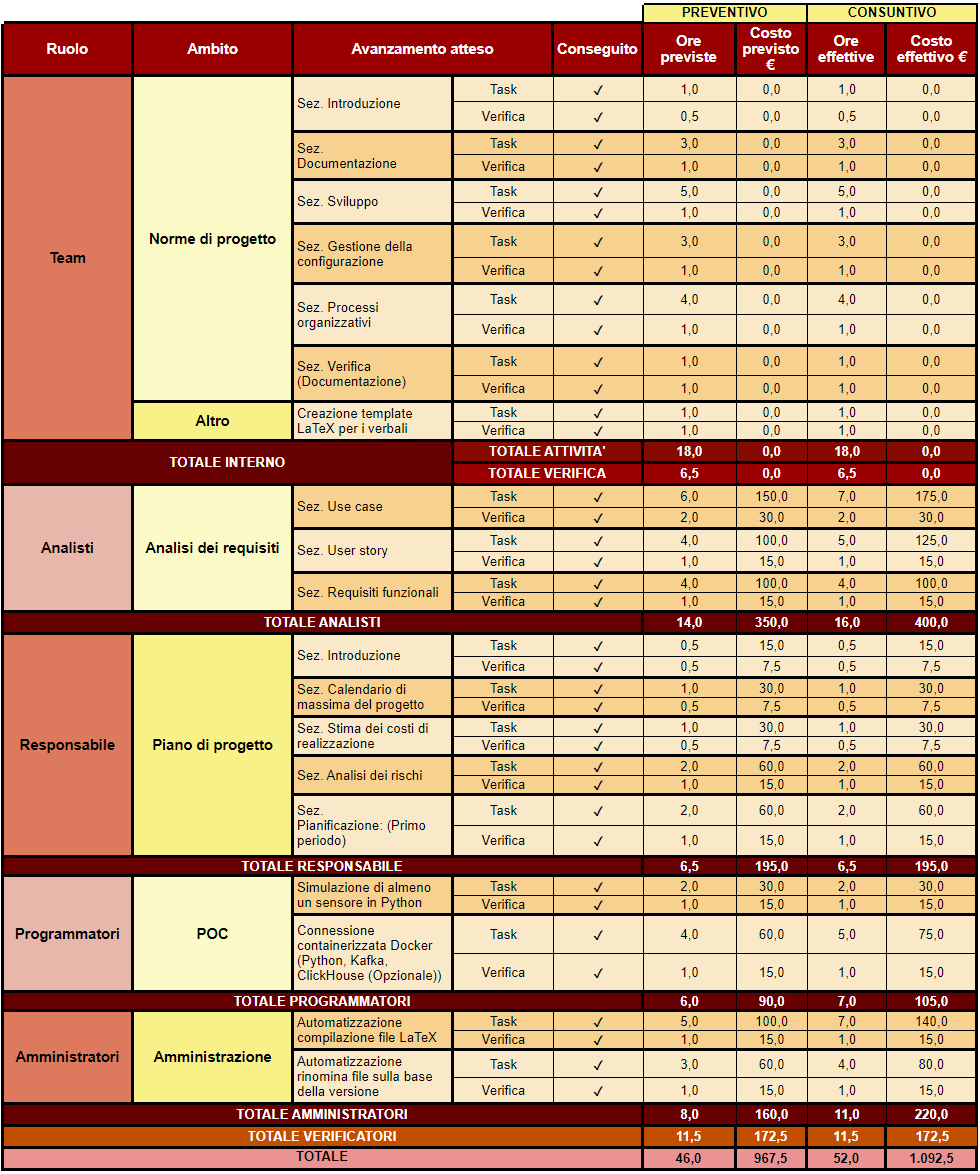
\includegraphics[height=0.9\textwidth]{../Images/periodo1.PNG}
    \caption{Primo periodo}
    \label{fig:Primo_periodo}
\end{figure}


Al termine del primo periodo, l'ammontare totale del costo del progetto è \textbf{ 1317,50\euro\ } e sono state completate il \textbf{100\%} delle \textit{attività}\textsubscript{\textit{G}} attese.
Il preventivo a finire rimane invariato a \textbf{12565,00€} e non risulta necessaria una ripianificazione delle \textit{attività}\textsubscript{\textit{G}} future.
\href{https://github.com/orgs/ByteOps-swe/projects/3/views/1?sortedBy%5Bdirection%5D=asc&sortedBy%5BcolumnId%5D=64182560}{Vai al Diagramma di Gantt.}

\pagebreak

\begin{figure}[H]
    \centering
    \begin{minipage}[b]{0.70\textwidth}
        \centering
        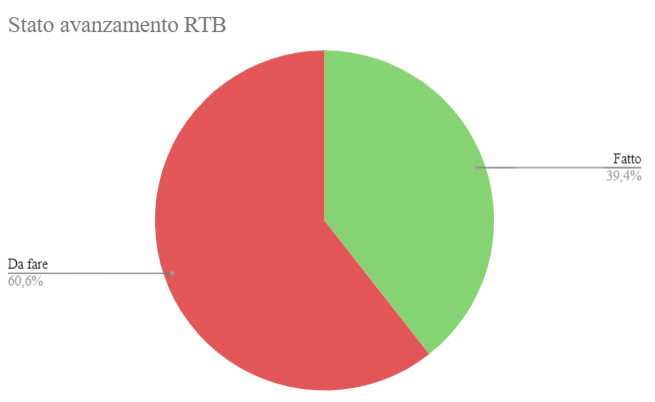
\includegraphics[width=0.7\textwidth]{../Images/avanzamento1Periodo.png}
        \caption{Avanzamento dei lavori RTB - Primo periodo}
        \label{fig:Avanzamento_RTB_1}
    \end{minipage}
\end{figure}

\paragraph{Preventivo orario}

\begin{figure}[H] 
    \centering
    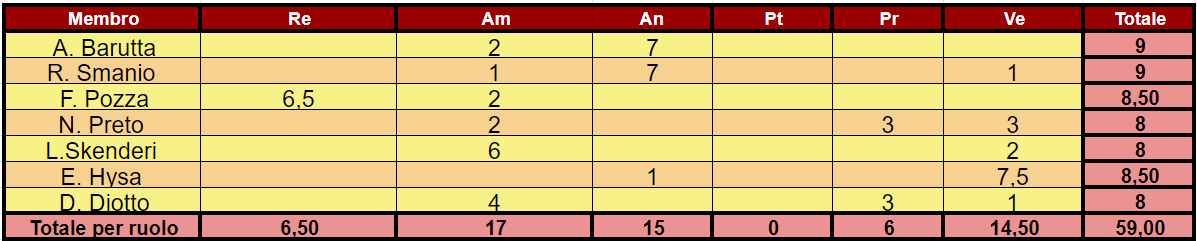
\includegraphics[width=0.9\textwidth]{../Images/preventivoOrario1Periodo.png}
    \caption{Preventivo orario per membro - Primo periodo}
    \label{fig:Preventivo_orario_1}
\end{figure}

\vspace{0.6cm}

\begin{figure}[H]
    \centering
    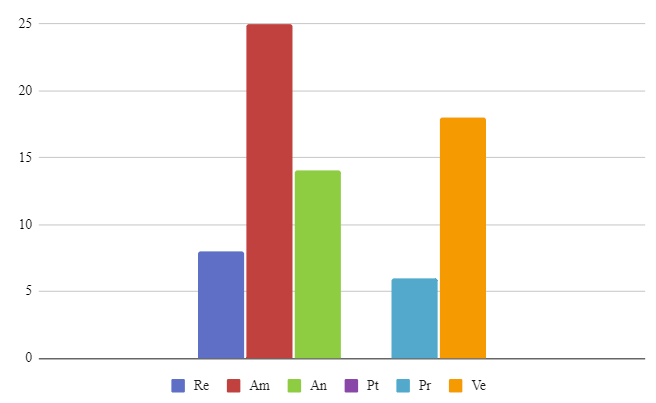
\includegraphics[width=0.6\textwidth]{../Images/preventivoDivisioneRuoli1Periodo.png}
    \caption{Istogramma preventivo della ripartizione oraria dei ruoli - Primo periodo}
    \label{fig:Preventivo_ripartizione_oraria_1}
\end{figure}

\pagebreak

\paragraph{Consuntivo orario}

\begin{figure}[H]
    \centering
    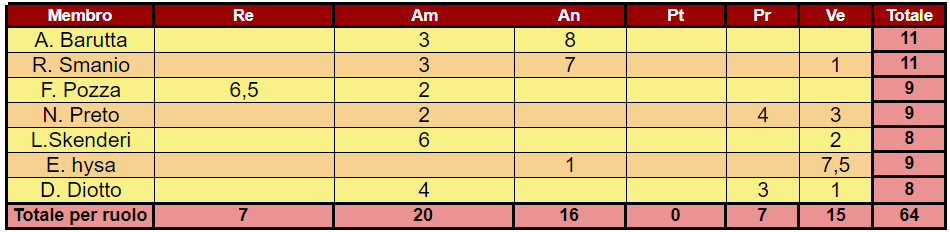
\includegraphics[width=0.9\textwidth]{../Images/consuntivoOrario1Periodo.png}
    \caption{Consuntivo orario per membro - Primo periodo}
    \label{fig:Constuntivo_orario_1}
\end{figure}

\vspace{0.6cm}

\begin{figure}[H]
    \centering
    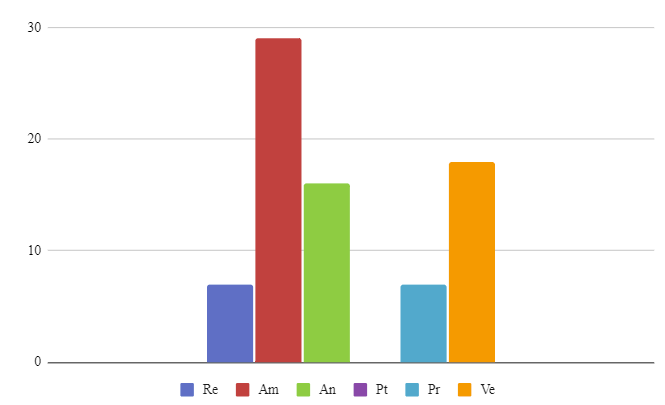
\includegraphics[width=0.6\textwidth]{../Images/consuntivoDivisioneRuoli1Periodo.png}
    \caption{Istogramma consuntivo della ripartizione oraria dei ruoli - Primo periodo}
    \label{fig:Consuntivo_ripartizione_oraria_1}
\end{figure}

%________________________-SECONDO PERIODO-_____________________________

\subsubsection{Secondo periodo  24/11/2023 - 08/12/2023}
\paragraph{Considerazioni}

Durante il secondo periodo, il nostro team ha impegnato risorse per proseguire e completare parzialmente la definizione delle norme nel documento \textit{Norme di Progetto}.

Durante questo periodo, sono state impiegate ore dei progettisti per prendere in considerazione tecnologie al di fuori di quelle consigliate dal \textit{proponente}\textsubscript{\textit{G}} e valutare diverse scelte architetturali.

Di fatto, è stato deciso di aggiungere un ulteriore passaggio allo \textit{stack tecnologico}\textsubscript{\textit{G}}, consistente in uno \textit{script}\textsubscript{\textit{G}} tra \textit{Kafka}\textsubscript{\textit{G}} e \textit{ClickHouse}\textsubscript{\textit{G}}, mirato a filtrare i dati provenienti dai sensori, evitando il salvataggio di errori di misurazione evidenti e consentendo il calcolo del punteggio di salute tramite una funzione di aggregazione.

\vspace{0.2cm}

Nel corso del \textit{SAL}\textsubscript{\textit{G}} con il \textit{proponente}\textsubscript{\textit{G}}, è stato stabilito l'obiettivo di integrare entro la fine del secondo sprint l'ultimo elemento dello \textit{stack tecnologico}\textsubscript{\textit{G}} del Proof of Concept (\textit{POC}\textsubscript{\textit{G}}) ovvero "\textit{Grafana}\textsubscript{\textit{G}}", e di inserire la funzionalità visualizzazione di grafici delle misurazioni dei simulatori sviluppati.

\vspace{0.2cm}

È soddisfacente constatare che tutte le richieste del \textit{proponente}\textsubscript{\textit{G}} sono state risolte entro i tempi concordati, portando così a buon punto lo sviluppo del \textit{POC}\textsubscript{\textit{G}}.

Successivamente a un colloquio con il Prof. Cardin e al suo reindirizzamento sui casi d'uso, gli analisti hanno ridefinito parte di essi, causando un arretramento nel progresso verso la conclusione della \textit{RTB}\textsubscript{\textit{G}}.

\vspace{0.2cm}

L'amministratore ha redatto il Glossario di progetto e definito gli \textit{standard}\textsubscript{\textit{G}} e le metriche di qualità di processo e prodotti nel documento \textit{Piano di qualifica}.

\paragraph{Gestione dei rischi} 

%Nel corso del secondo periodo, ci si attendeva e si sono manifestate le seguenti problematiche:
\begin{itemize}
    \item \textbf{Rischi attesi e verificati:}
\begin{itemize}
    \item \textbf{RO-1A-1} - Assenza di uno dei membri per 4 giorni~(\textit{\ref{sec:ImpPersonali}})
    \begin{itemize}
        \item \textbf{Esito mitigazione:} 
        l'azione di mitigazione adottata si è dimostrata efficace, senza suscitare proposte di modifiche;
        \item \textbf{Impatto:}
        non sono emerse conseguenze significative. Conformemente al processo di mitigazione, il responsabile ha ridistribuito i compiti del membro assente assegnandoli a ruoli con un carico lavorativo ridotto durante il periodo di assenza del membro.
    \end{itemize}
\end{itemize}
\item \textbf{Rischi attesi ma non verificati:}
 \begin{itemize}
    \item \textbf{RT-1A-1} - Apprendimento ed utilizzo delle nuove tecnologie~(\textit{\ref{sec:rischioTec}});
    \item \textbf{RO-2M-2} - Ritardo nel completamento delle \textit{attività}\textsubscript{\textit{G}} rispetto ai tempi previsti~(\textit{\ref{sec:ritAttivita}});
    \item \textbf{RP-2B-1} - Contrasti interni al gruppo~(\textit{\ref{subsubsec:contrastiInterni}}).
\end{itemize}
\item \textbf{Rischi non attesi ma verificati:}
\begin{itemize}
    \item Nessuno.
\end{itemize}
\end{itemize}

\pagebreak

\paragraph{Definizione ruoli}
Durante questo periodo diversi membri hanno assunto più ruoli per poter portare a termine tutte le \textit{attività}\textsubscript{\textit{G}} pianificate.
Per le \textit{attività}\textsubscript{\textit{G}} registrate nei costi, sono stati assegnati i seguenti ruoli:

\vspace{0.4cm}

\begin{table}[H]
    \centering
    \begin{tabular}{|L{4cm}|L{2cm}|}
    \hline
    \textbf{Ruolo} & \textbf{Persona} \\
    \hline
    \hline
    Responsabile (Re)   & L. Skenderi \\
    \hline
    Amministratore (Am) & A. Barutta \\
    \hline
    Analisti (An)       & E. Hysa \\
                        & R. Smanio \\
    \hline
    Verificatore (Ve)   & D. Diotto \\
                        & R. Smanio \\
    \hline
    Programmatori (Pr)  & N. Preto \\
                        & F. Pozza \\
    \hline
    Progettista (Pt)    & A. Barutta \\
                        & F. Pozza \\
                        & R. Smanio \\
                        & L. Skenderi \\
                        & E. Hysa \\
    \hline
    \end{tabular}
    \caption{Tabella dei ruoli assegnati - Secondo periodo}
    \label{tab:Ruoli_persone_2}
    \end{table}
    
\newpage
\paragraph{Pianificazione attività divise per ruoli con consuntivo e preventivo orario e dei costi}

\begin{figure}[H]
    \centering
    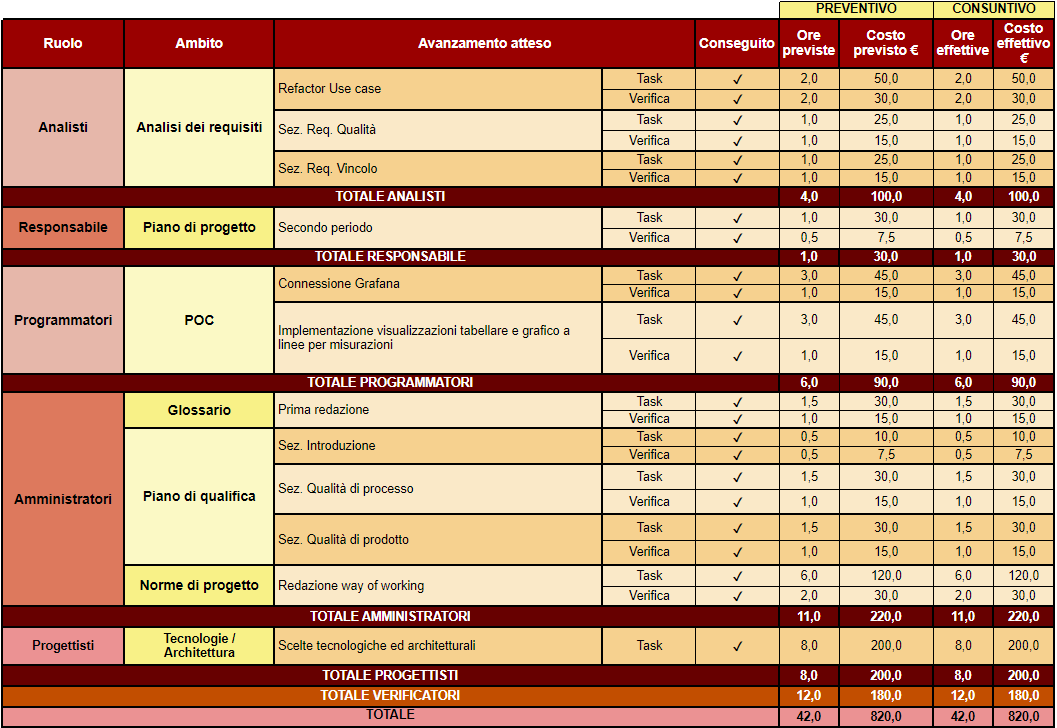
\includegraphics[width=\linewidth, height=0.9\textheight, keepaspectratio]{../Images/periodo2.PNG}
    \caption{Secondo periodo}
    \label{fig:Secondo_periodo}
\end{figure}

\vspace{1cm}

Al termine del secondo periodo, l'ammontare totale del costo del progetto è \textbf{2137,50\euro\ } e sono state completate il \textbf{100\%} delle \textit{attività}\textsubscript{\textit{G}} attese.
Il preventivo a finire rimane invariato a \textbf{12565,00€} e non risulta necessaria una ripianificazione delle \textit{attività}\textsubscript{\textit{G}} future.
\href{https://github.com/orgs/ByteOps-swe/projects/3/views/1?sortedBy%5Bdirection%5D=asc&sortedBy%5BcolumnId%5D=64182560}{Vai al Diagramma di Gantt.}


\begin{figure}[H]
    \centering
    \begin{minipage}[b]{0.70\textwidth}
        \centering
        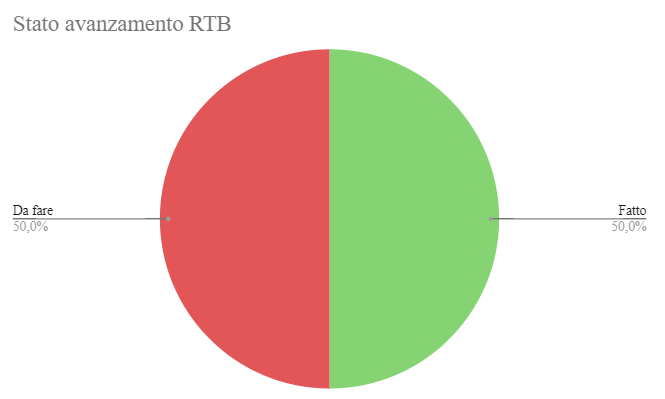
\includegraphics[width=0.7\textwidth]{../Images/avanzamento2Periodo.png}
        \caption{Avanzamento dei lavori RTB - Secondo periodo}
        \label{fig:Avanzamento_RTB_2}
    \end{minipage}
\end{figure}



\paragraph{Preventivo orario}

\begin{figure}[H]
    \centering
    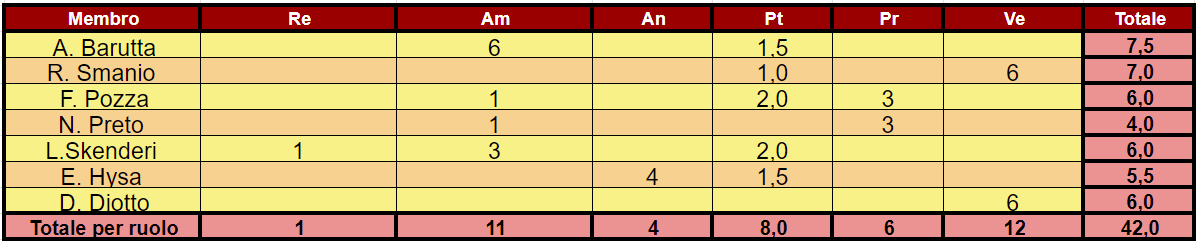
\includegraphics[width=0.9\textwidth]{../Images/preventivoOrario2Periodo.png}
    \caption{Preventivo orario per membro - Secondo periodo}
    \label{fig:Preventivo_orario_2}
\end{figure}

\vspace{0.6cm}

\begin{figure}[H]
    \centering
    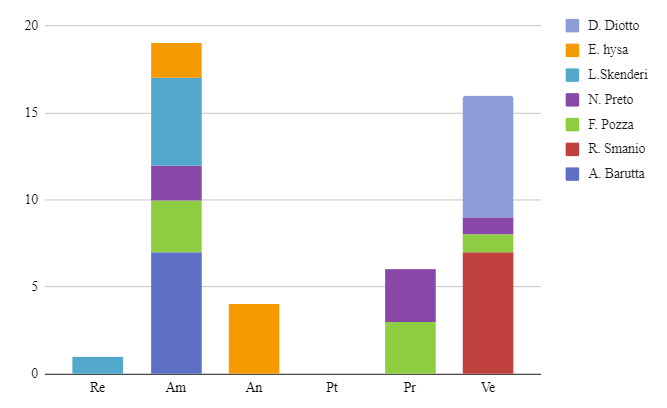
\includegraphics[width=0.6\textwidth]{../Images/preventivoDivisioneRuoli2Periodo.png}
    \caption{Istogramma preventivo della ripartizione oraria dei ruoli - Secondo periodo}
    \label{fig:Preventivo_ripartizione_oraria_2}
\end{figure}

\paragraph{Consuntivo orario } 

\begin{figure}[H]
    \centering
    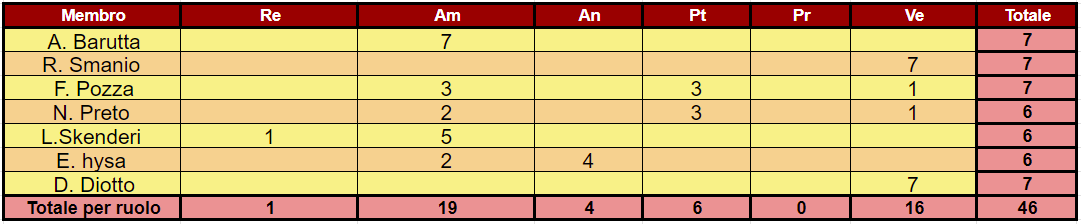
\includegraphics[width=0.9\textwidth]{../Images/consuntivoOrario2Periodo.png}
    \caption{Consuntivo orario per membro - Secondo periodo}
    \label{fig:Constuntivo_orario_2}
\end{figure}

\vspace{0.6cm}

\begin{figure}[H]
    \centering
    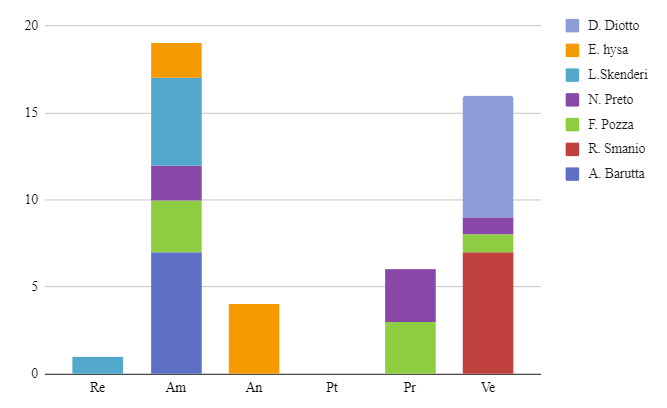
\includegraphics[width=0.6\textwidth]{../Images/consuntivoDivisioneRuoli2Periodo.png}
    \caption{Istogramma consuntivo della ripartizione oraria dei ruoli - Secondo periodo}
    \label{fig:Consuntivo_ripartizione_oraria_2}
\end{figure}


%________________________-TERZO PERIODO-_____________________________


\subsubsection{Terzo periodo  08/12/2023 - 21/12/2023}
\paragraph{Considerazioni}
Nel corso del terzo periodo, il nostro team ha allocato risorse significative per condurre una revisione esaustiva del documento \textit{Norme di Progetto}.

\vspace{0.2cm}

L'amministratore si è concentrato sulla redazione del \textit{Piano di qualifica}, nonché sulla definizione e revisione delle metriche di qualità. 

\vspace{0.2cm}

Gli analisti hanno completato il refactoring completo del documento \textit{Analisi dei requisiti}, includendo la conclusione dei casi d'uso, dei requisiti funzionali, dei requisiti di vincolo, dei requisiti di qualità e del tracciamento.

\vspace{0.2cm}

I programmatori hanno dedicato un impegno considerevole alla risoluzione di bug nel Proof of Concept (\textit{POC}\textsubscript{\textit{G}}) e alla creazione di una versione stabile destinata alla presentazione durante la revisione \textit{RTB}\textsubscript{\textit{G}}.

\paragraph{Gestione dei rischi} 

\begin{itemize}
    \item \textbf{Rischi attesi e verificati:}
\begin{itemize}
    \item Nessuno.
\end{itemize}
\item \textbf{Rischi attesi ma non verificati:}
 \begin{itemize}
    \item \textbf{RT-1A-1} - Apprendimento ed utilizzo delle nuove tecnologie~(\textit{\ref{sec:rischioTec}});
    \item \textbf{RO-2M-2} - Ritardo nel completamento delle \textit{attività}\textsubscript{\textit{G}} rispetto ai tempi previsti~(\textit{\ref{sec:ritAttivita}}).
\end{itemize}
\item \textbf{Rischi non attesi ma verificati:}
\begin{itemize}
    \item Nessuno.
\end{itemize}
\end{itemize}
\paragraph{Definizione ruoli} 
Per le \textit{attività}\textsubscript{\textit{G}} registrate nei costi, sono stati assegnati i seguenti ruoli:  

\vspace{0.4cm}

\begin{table}[H]
    \centering
    \begin{tabular}{|L{4cm}|L{2cm}|}
    \hline
    \textbf{Ruolo} & \textbf{Persona} \\
    \hline
    \hline
    Responsabile (Re)   & R. Smanio \\
    \hline
    Amministratore (Am) & D. Diotto \\
    \hline
    Analisti (An)       & L. Skenderi \\
    \hline
    Verificatore (Ve)   & N. Preto \\
                        & A. Barutta \\
    \hline
    Programmatori (Pr)  & E. Hysa \\
                        & F. Pozza \\
    \hline
    Progettista (Pt)    & Nessuno \\
    \hline
    \end{tabular}
    \caption{Tabella dei ruoli assegnati - Terzo periodo}
    \label{tab:Ruoli_persone_3}
    \end{table}

\newpage
\paragraph{Pianificazione attività divise per ruoli con consuntivo e preventivo orario e dei costi}

\begin{figure}[H]
    \centering
    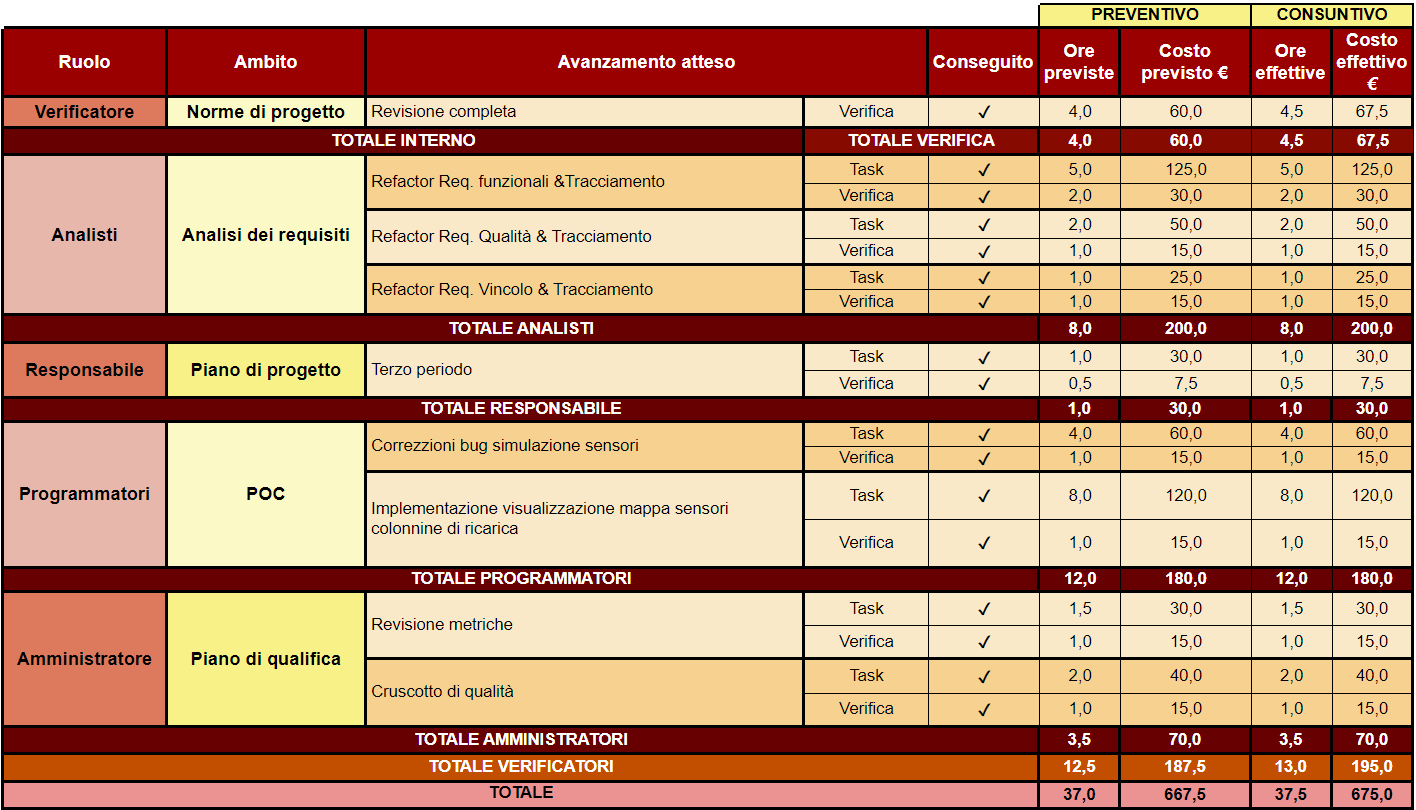
\includegraphics[width=\linewidth, height=0.9\textheight, keepaspectratio]{../Images/periodo3.PNG}
    \caption{Terzo periodo}
    \label{fig:Terzo_periodo}
\end{figure}

\vspace{0.5cm}

Al termine del terzo periodo, l'ammontare totale del costo del progetto è \textbf{ 2812,5\euro\ } e sono state completate il \textbf{100\%} delle \textit{attività}\textsubscript{\textit{G}} attese.
Il preventivo a finire rimane invariato a \textbf{12565,00€} e non risulta necessaria una ripianificazione delle \textit{attività}\textsubscript{\textit{G}} future.
\href{https://github.com/orgs/ByteOps-swe/projects/3/views/1?sortedBy%5Bdirection%5D=asc&sortedBy%5BcolumnId%5D=64182560}{Vai al Diagramma di Gantt.}

\pagebreak

\begin{figure}[H]
    \centering
    \begin{minipage}[b]{0.70\textwidth}
        \centering
        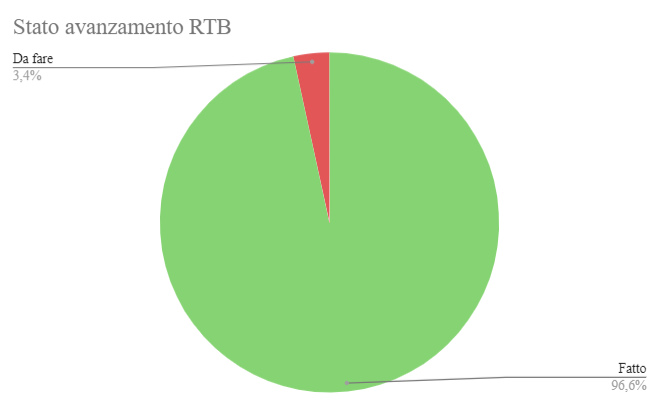
\includegraphics[width=0.7\textwidth]{../Images/avanzamento3Periodo.png}
        \caption{Avanzamento dei lavori RTB - Terzo periodo}
        \label{fig:Avanzamento_RTB_3}
    \end{minipage}
\end{figure}

\paragraph{Preventivo orario} 

\begin{figure}[H]
    \centering
    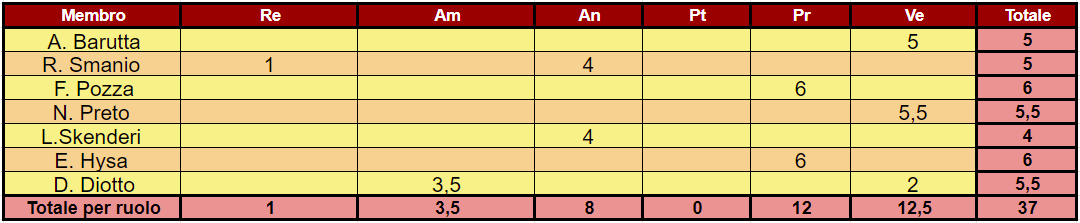
\includegraphics[width=0.9\textwidth]{../Images/preventivoOrario3Periodo.png}
    \caption{Preventivo orario per membro - Terzo periodo}
    \label{fig:Preventivo_orario_3}
\end{figure}

\vspace{0.4cm}

\begin{figure}[H]
    \centering
    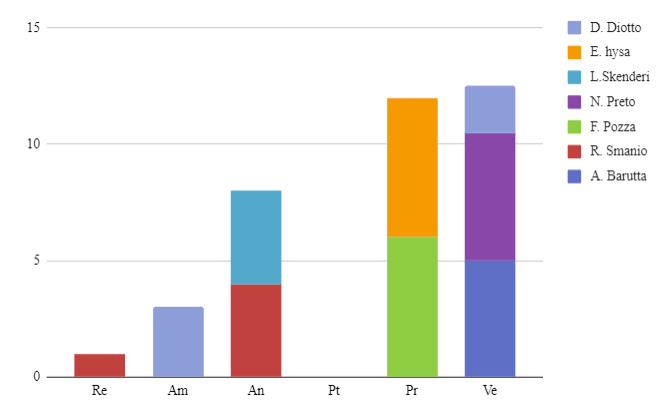
\includegraphics[width=0.6\textwidth]{../Images/preventivoDivisioneRuoli3Periodo.png}
    \caption{Istogramma preventivo della ripartizione oraria dei ruoli - Terzo periodo}
    \label{fig:Preventivo_ripartizione_oraria_3}
\end{figure}

\paragraph{Consuntivo orario} 

\begin{figure}[H]
    \centering
    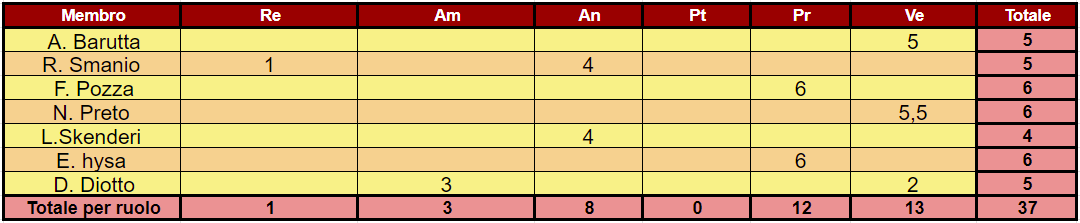
\includegraphics[width=0.9\textwidth]{../Images/consuntivoOrario3Periodo.png}
    \caption{Consuntivo orario per membro - Terzo periodo}
    \label{fig:Constuntivo_orario_3}
\end{figure}

\vspace{0.6cm}

\begin{figure}[H]
    \centering
    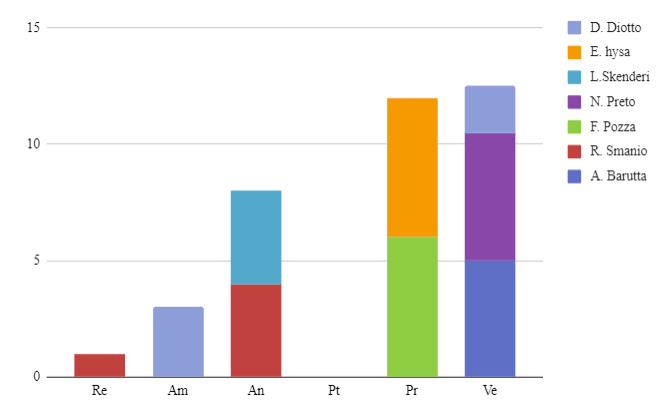
\includegraphics[width=0.6\textwidth]{../Images/consuntivoDivisioneRuoli3Periodo.png}
    \caption{Istogramma consuntivo della ripartizione oraria dei ruoli - Terzo periodo}
    \label{fig:Consuntivo_ripartizione_oraria_3}
\end{figure}


%________________________-QUARTO PERIODO-_____________________________


\subsubsection{Quarto periodo  21/12/2023 - 07/01/2024}
\paragraph{Considerazioni}
Il quarto periodo è stato principalmente sul perfezionamento del documento di \textit{Analisi dei Requisiti}\textsubscript{\textit{G}}. Ciò ha comportato un miglioramento delle descrizioni dei casi d'uso, delle user stories, dei requisiti e del tracciamento di quest'ultimi.

Le \textit{attività}\textsubscript{\textit{G}} di programmazione si sono svolte mirando a garantire solidità ed efficienza del prodotto (\textit{POC}\textsubscript{\textit{G}}) in vista della revisione \textit{RTB}\textsubscript{\textit{G}}. 
Inoltre, è stata creata una pagina su GitHub.io per consentire una navigazione chiara e rapida della \textit{repository}\textsubscript{\textit{G}} del progetto.

Durante questo periodo, sono state istanziate rilevanti risorse per condurre \textit{attività}\textsubscript{\textit{G}} di verifica generale su tutti i \textit{configuration item}\textsubscript{\textit{G}} prodotti nel corso dei quattro periodi.

\paragraph{Gestione dei rischi} 
\begin{itemize}
    \item \textbf{Rischi attesi e verificati:}
\begin{itemize}
    \item \textbf{RO-1A-1} - Rallentamento del progetto dovuto all'occorrenza delle \textit{attività}\textsubscript{\textit{G}} personali~(\textit{\ref{sec:ImpPersonali}}).
    \begin{itemize}
        \item \textbf{Esito mitigazione:}
            il responsabile in accordo con la \textit{proponente}\textsubscript{\textit{G}} ha prudentemente vincolato il numero di \textit{attività}\textsubscript{\textit{G}} avviate durante questo periodo, estendendone i tempi, al fine di assicurarne il completo svolgimento;
        \item \textbf{Impatto:}
            in vista dell'imminente avvio della sessione invernale, si è verificato un rallentamento delle \textit{attività}\textsubscript{\textit{G}} a causa degli impegni accademici dei membri del team.
    \end{itemize}
\end{itemize}
\item \textbf{Rischi attesi ma non verificati:}
 \begin{itemize}
    \item Nessuno.
\end{itemize}
\item \textbf{Rischi non attesi ma verificati:}
\begin{itemize}
    \item Nessuno.
\end{itemize}
\end{itemize}

\paragraph{Definizione ruoli} 
Per le \textit{attività}\textsubscript{\textit{G}} registrate nei costi, sono stati assegnati i seguenti ruoli: (durante tale periodo, alcuni membri del team hanno assunto più responsabilità, conformemente a quanto concordato sin dall'inizio del periodo).

\vspace{0.4cm}

\begin{table}[H]
    \centering
    \begin{tabular}{|L{4cm}|L{2cm}|}
    \hline
    \textbf{Ruolo} & \textbf{Persona} \\
    \hline
    \hline
    Responsabile (Re)   & N. Preto \\
    \hline
    Amministratore (Am) & E. Hysa \\
    \hline
    Analisti (An)       & F. Pozza \\
                        & D. Diotto \\
    \hline
    Verificatore (Ve)   & L. Skenderi \\
                        & N. Preto \\
                        & E. Hysa \\
     \hline
    Programmatori (Pr)  & A. Barutta \\
                        & R. Smanio \\
    \hline
    Progettista (Pt)    & Nessuno \\
    \hline
    \end{tabular}
    \caption{Tabella dei ruoli assegnati - Quarto periodo}
    \label{tab:Ruoli_persone_4}
    \end{table}
    
\newpage
\paragraph{Pianificazione attività divise per ruoli con consuntivo e preventivo orario e dei costi}

\begin{figure}[H]
    \centering
    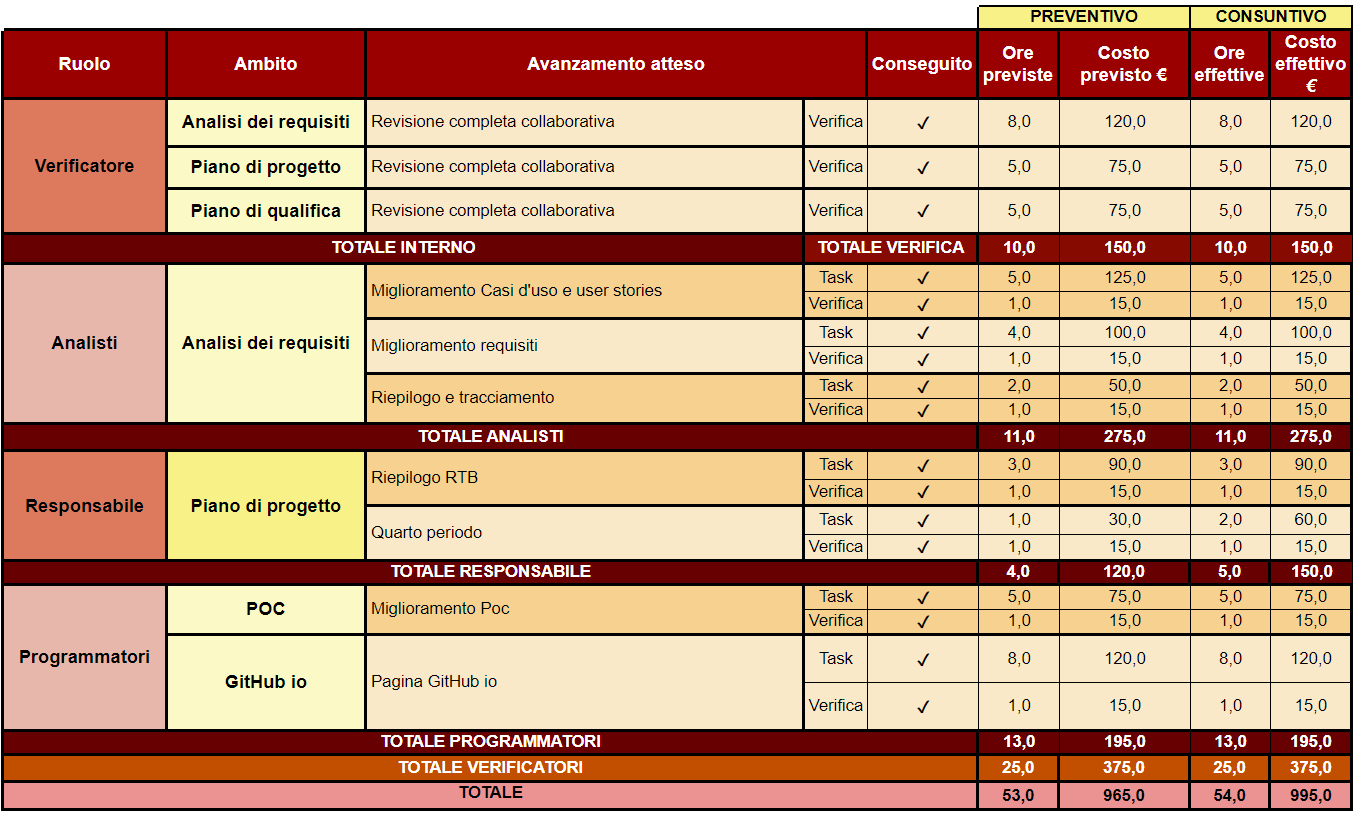
\includegraphics[width=\linewidth, height=0.9\textheight, keepaspectratio]{../Images/periodo4.PNG}
    \caption{Quarto periodo}
    \label{fig:Quarto_periodo}
\end{figure}

\vspace{1cm}

Al termine del quarto periodo, l'ammontare totale del costo del progetto è \textbf{ 3807,5\euro\ } e sono state completate il \textbf{100\%} delle \textit{attività}\textsubscript{\textit{G}} attese.
Il preventivo a finire rimane invariato a \textbf{12565,00€} e non risulta necessaria una ripianificazione delle \textit{attività}\textsubscript{\textit{G}} future.
\href{https://github.com/orgs/ByteOps-swe/projects/3/views/1?sortedBy%5Bdirection%5D=asc&sortedBy%5BcolumnId%5D=64182560}{Vai al Diagramma di Gantt.}

\pagebreak

\begin{figure}[H]
    \centering
    \begin{minipage}[b]{0.70\textwidth}
        \centering
        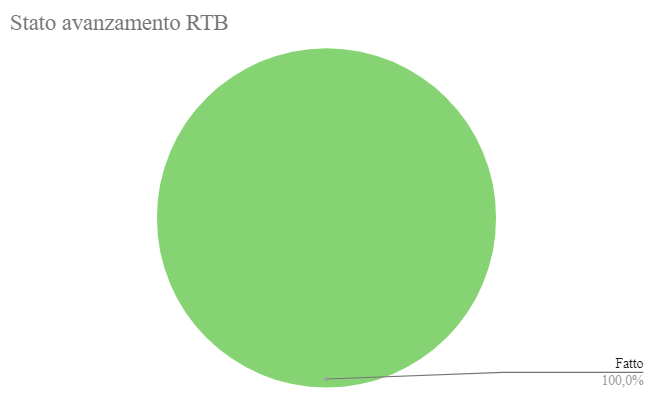
\includegraphics[width=0.7\textwidth]{../Images/avanzamento4Periodo.png}
        \caption{Avanzamento dei lavori RTB - Quarto periodo}
        \label{fig:Avanzamento_RTB_4}
    \end{minipage}
\end{figure}

\paragraph{Preventivo orario} 

\begin{figure}[H]
    \centering
    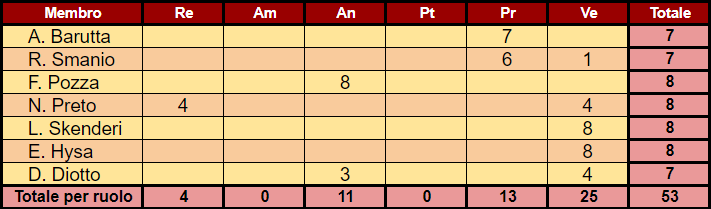
\includegraphics[width=0.9\textwidth]{../Images/preventivoOrario4Periodo.png}
    \caption{Preventivo orario per membro - Quarto periodo}
    \label{fig:Preventivo_orario_4}
\end{figure}

\vspace{0.6cm}

\begin{figure}[H]
    \centering
    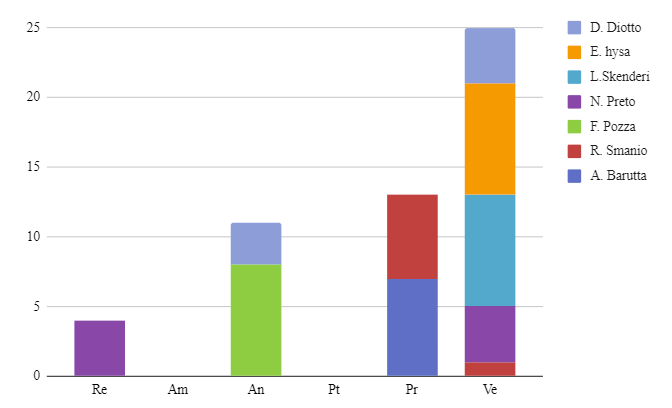
\includegraphics[width=0.6\textwidth]{../Images/preventivoDivisioneRuoli4Periodo.png}
    \caption{Istogramma preventivo della ripartizione oraria dei ruoli - Quarto periodo}
    \label{fig:Preventivo_ripartizione_oraria_4}
\end{figure}

\paragraph{Consuntivo orario} 

\begin{figure}[H]
    \centering
    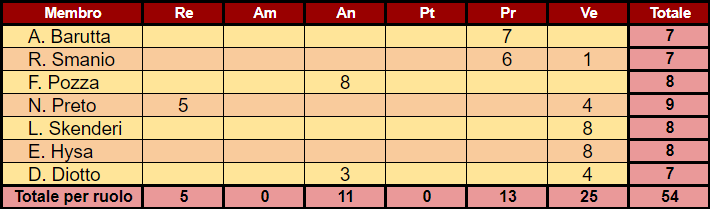
\includegraphics[width=0.9\textwidth]{../Images/consuntivoOrario4Periodo.png}
    \caption{Consuntivo orario per membro - Quarto periodo}
    \label{fig:Constuntivo_orario_4}
\end{figure}

\vspace{0.4cm}

\begin{figure}[H]
    \centering
    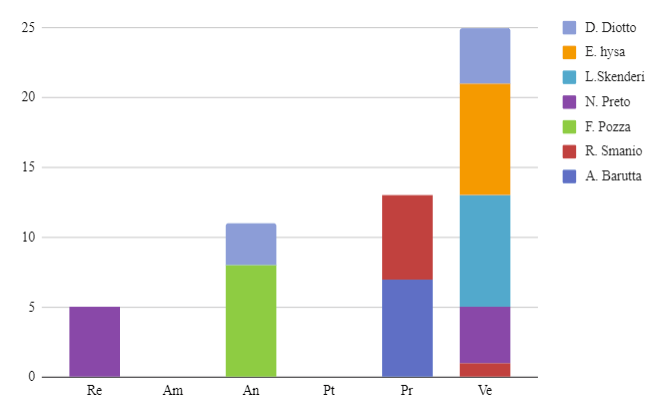
\includegraphics[width=0.6\textwidth]{../Images/consuntivoDivisioneRuoli4Periodo.png}
    \caption{Istogramma consuntivo della ripartizione oraria dei ruoli - Quarto periodo}
    \label{fig:Consuntivo_ripartizione_oraria_4}
\end{figure}

%________________________-QUINTO PERIODO-_____________________________


\subsubsection{Quinto periodo  07/01/2024 - 15/01/2024}
\paragraph{Considerazioni}
Durante il quinto periodo il team ha impiegato risorse per sviluppare le presentazioni sia per la parte relativa al professor Cardin che per quella relativa al professor Vardanega.

\vspace{0.2cm}

È importante notare che questo compito eseguito dagli amministratori e le risorse ad esso allocate non sono state incluse nel calcolo dei costi e nel consuntivo orario di progetto. 
In aggiunta, sono stati apportati lievi ritocchi di formalizzazione ai documenti.

\vspace{0.2cm}

Al termine del periodo è stato riscontrato il completamento delle \textit{attività}\textsubscript{\textit{G}} richieste per la revisione \textit{RTB}\textsubscript{\textit{G}}.

\pagebreak

\paragraph{Gestione dei rischi} 
\begin{itemize}
    \item \textbf{Rischi attesi e verificati:}
\begin{itemize}
    \item \textbf{RO-1A-1} - Rallentamento del progetto dovuto all'occorrenza delle \textit{attività}\textsubscript{\textit{G}} personali~(\textit{\ref{sec:ImpPersonali}}).
    \begin{itemize}
        \item \textbf{Esito mitigazione:} 
        in seguito a una concorde decisione tra il responsabile e la \textit{proponente}\textsubscript{\textit{G}}, è stato prudentemente limitato il numero di \textit{attività}\textsubscript{\textit{G}} avviate durante questo periodo. Ulteriormente, considerando l'avvicinarsi della sessione invernale di esami, si è provveduto a ridurre l'ampiezza temporale a una settimana;
        \item \textbf{Impatto:}
        l'avanzamento procede a ritmo più lento, tuttavia tale andamento è conforme a quanto preventivato durante la fase di pianificazione.
    \end{itemize}
\end{itemize}
\item \textbf{Rischi attesi ma non verificati:}
 \begin{itemize}
    \item Nessuno.
\end{itemize}
\item \textbf{Rischi non attesi ma verificati:}
\begin{itemize}
    \item Nessuno.
\end{itemize}
\end{itemize}

\paragraph{Definizione ruoli}
Per le \textit{attività}\textsubscript{\textit{G}} registrate nei costi, sono stati assegnati i seguenti ruoli:

\vspace{0.4cm}

\begin{table}[H]
    \centering
    \begin{tabular}{|L{4cm}|L{2cm}|}
    \hline
    \textbf{Ruolo} & \textbf{Persona} \\
    \hline
    \hline
    Responsabile (Re)   & D. Diotto \\
    \hline
    Amministratore (Am) & A.Barutta  \\
                        & R. Smanio \\
    \hline
    Analisti (An)       & E. Hysa \\
                        & N. Preto \\
    \hline
    Verificatore (Ve)   & F. Pozza \\
                        & L. Skenderi\\
     \hline
    Programmatori (Pr)  & L. Skenderi \\    
    \hline
    Progettista (Pt)    & Nessuno \\
    \hline
    \end{tabular}
    \caption{Tabella dei ruoli assegnati - Quinto periodo}
    \label{tab:Ruoli_persone_5}
    \end{table}

\newpage
\paragraph{Pianificazione attività divise per ruoli con consuntivo e preventivo orario e dei costi}

\begin{figure}[H]
    \centering
    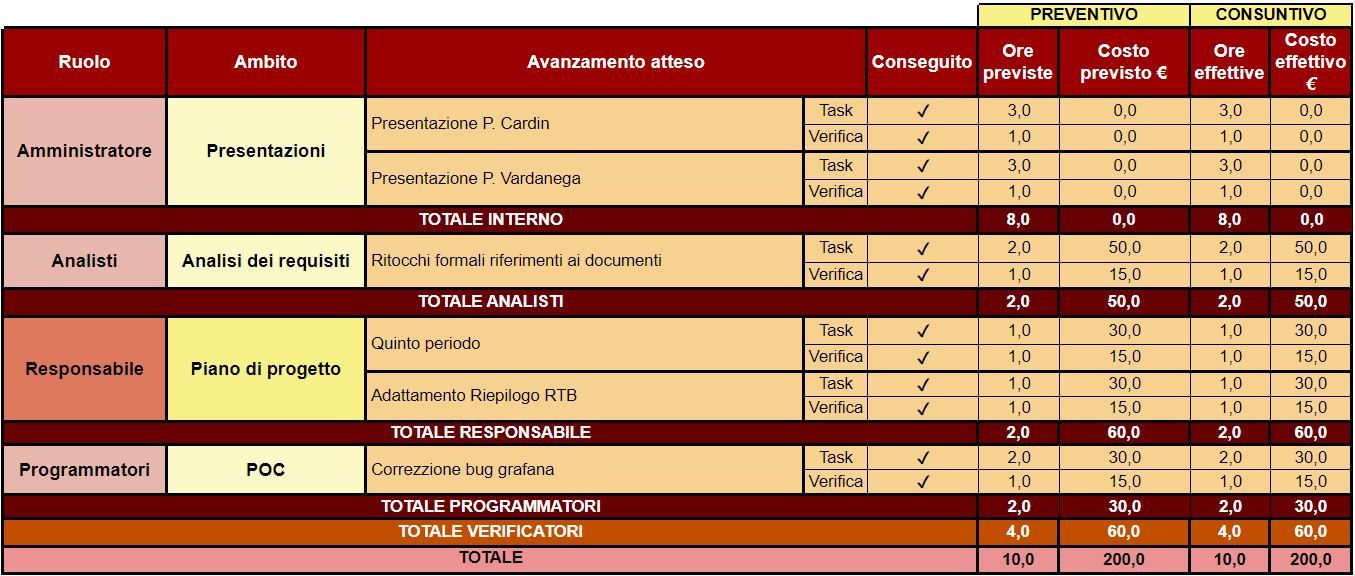
\includegraphics[width=\linewidth, height=0.9\textheight, keepaspectratio]{../Images/periodo5.PNG}
    \caption{quinto periodo}
    \label{fig:Quinto_periodo}
\end{figure}

\vspace{1cm}

Al termine del quinto periodo, l'ammontare totale del costo del progetto è \textbf{4007,50\euro\ } e sono state completate il \textbf{100\%} delle \textit{attività}\textsubscript{\textit{G}} attese.
Il preventivo a finire rimane invariato a \textbf{12565,00€} e non risulta necessaria una ripianificazione delle \textit{attività}\textsubscript{\textit{G}} future.

\pagebreak

\begin{figure}[H]
    \centering
    \begin{minipage}[b]{0.70\textwidth}
        \centering
        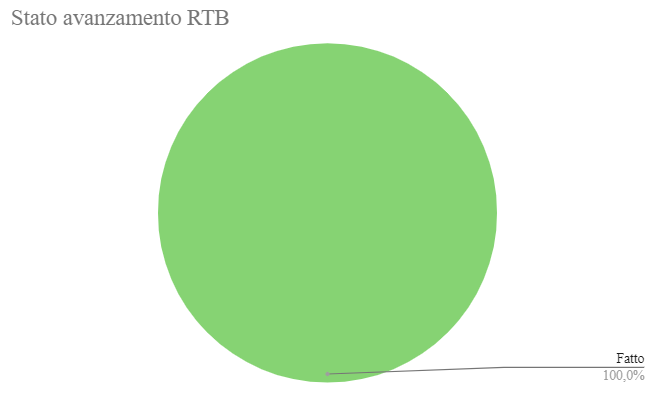
\includegraphics[width=0.7\textwidth]{../Images/avanzamento5Periodo.png}
        \caption{Avanzamento dei lavori RTB - Quinto periodo}
        \label{fig:Avanzamento_RTB_5}
    \end{minipage}
\end{figure}

\paragraph{Preventivo orario}

\begin{figure}[H]
    \centering
    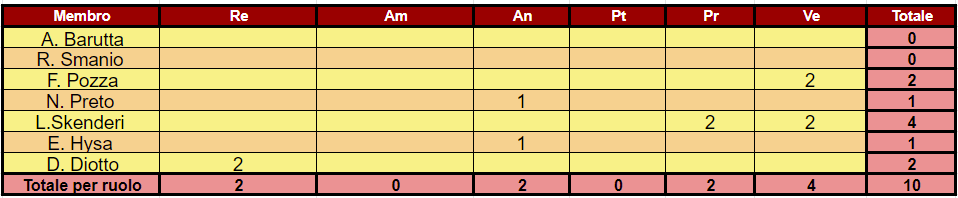
\includegraphics[width=0.9\textwidth]{../Images/preventivoOrario5Periodo.png}
    \caption{Preventivo orario per membro - Quinto periodo}
    \label{fig:Preventivo_orario_5}
\end{figure}

\vspace{0.6cm}

\begin{figure}[H] 
    \centering
    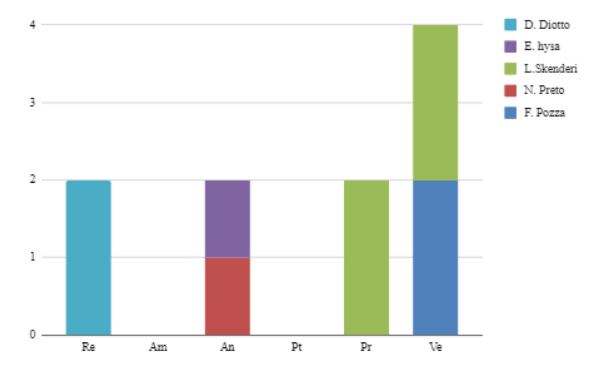
\includegraphics[width=0.6\textwidth]{../Images/preventivoDivisioneRuoli5Periodo.png}
    \caption{Istogramma preventivo della ripartizione oraria dei ruoli - Quinto periodo}
    \label{fig:Preventivo_ripartizione_oraria_5}
\end{figure} 

\paragraph{Consuntivo orario}

\begin{figure}[H]
    \centering
    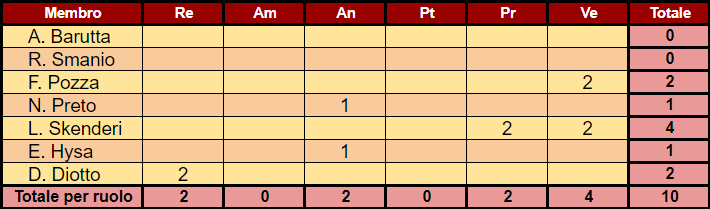
\includegraphics[width=0.9\textwidth]{../Images/consuntivoOrario5Periodo.png}
    \caption{Consuntivo orario per membro - Quinto periodo}
    \label{fig:Constuntivo_orario_5}
\end{figure}

\begin{figure}[H]
    \centering
    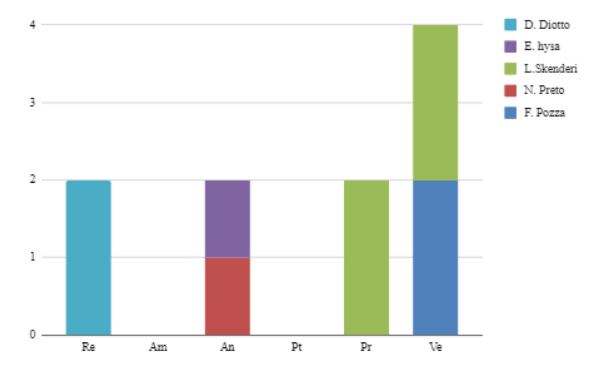
\includegraphics[width=0.6\textwidth]{../Images/consuntivoDivisioneRuoli5Periodo.png}
    \caption{Istogramma consuntivo della ripartizione oraria dei ruoli - Quinto periodo}
    \label{fig:Consuntivo_ripartizione_oraria_5}
\end{figure}
%________________________-Sesto PERIODO-_____________________________


\subsubsection{Sesto periodo  15/01/2024 - 01/02/2024}
\paragraph{Pianificazione}
Per quanto attiene all'organizzazione di questo periodo, in considerazione della sovrapposizione con l'inizio della sessione di esami, il gruppo ha unanimemente raggiunto un accordo.

Oltre a dedicarsi alla preparazione per i colloqui della \textit{RTB}\textsubscript{\textit{G}}, si è deliberato di focalizzarsi principalmente sullo studio individuale necessario per affrontare la sessione stessa, evitando ulteriori avanzamenti nel progetto.

\vspace{0.2cm}

In questo periodo quindi, ci dedicheremo esclusivamente alla rifinitura dei dettagli concernenti le presentazioni destinate al Prof. Cardin e al Prof. Vardanega.

\paragraph{Considerazioni}
Durante questo periodo, dopo un'analisi delle \textit{attività}\textsubscript{\textit{G}} svolte fino a questo momento e delle ore impiegate dai vari ruoli, è emersa la necessità di modificare la pianificazione delle ore lavorative per i membri, poiché si è constatato che gli amministratori hanno un numero di ore insufficiente rispetto alle \textit{attività}\textsubscript{\textit{G}} rimanenti, mentre i responsabili ne hanno un eccesso.

\vspace{0.2cm}

Il preventivo a finire è ora quindi di \textbf{12425,00€} data la ridistribuzione oraria visibile nella \textit{sezione~\ref{sec:TerzaStesura}} e la consegna finale del prodotto slitta al 25/03/2024, a causa del tempo dedicato allo studio per gli esami durante il periodo, come indicato nella \textit{sezione~\ref{sec:SecondaStesuraCalendario}}. 


\paragraph{Gestione dei rischi} 
\begin{itemize}
    \item \textbf{Rischi attesi e verificati:}
\begin{itemize}
    \item \textbf{RO-1A-1} - Rallentamento del progetto dovuto all'occorrenza delle \textit{attività}\textsubscript{\textit{G}} personali~(\textit{\ref{sec:ImpPersonali}}).
    \begin{itemize}
        \item \textbf{Impatto:}
       l'avanzamento del progetto è nullo in questo periodo, ma ciò è conforme a quanto preventivato
    \end{itemize}
\end{itemize}
\item \textbf{Rischi attesi ma non verificati:}
    \begin{itemize}
        \item Nessuno.
    \end{itemize}
    \item \textbf{Rischi non attesi ma verificati:}
    \begin{itemize}
        \item Nessuno.
    \end{itemize}
\end{itemize}
\newpage
\paragraph{Pianificazione attività, preventivo e consuntivo}
Non è previsto e pianificato avanzamento effettivo all’interno di questo periodo, se non per ciò che riguarda
le presentazioni relative alla \textit{RTB}\textsubscript{\textit{G}}.
Di conseguenza non vengono riportati preventivi e consuntivi di periodo.